
\newcommand{\nomedoc}{Specifica Tecnica}
\newcommand{\versione}{0.11}
\newcommand{\versioneglossario}{1.0}
\newcommand{\versionenormeprogetto}{1.0}
\newcommand{\nomefile}{SpecificaTecnica-\versione.pdf}
\newcommand{\datacreazione}{2 Dicembre 2010}
\newcommand{\datamodifica}{29 Gennaio 2011}
\newcommand{\stato}{formale}
\newcommand{\uso}{interno}
\newcommand{\redazione}{Mandolo Andrea}
\newcommand{\verifica}{---}
\newcommand{\approvazione}{---}
\newcommand{\distribuzione}{
VT.G \\
& Prof. Vardanega Tullio\\
& Prof. Cardin Riccardo }

% FUNZIONI TIPOGRAFICHE
\newcommand{\co}{\texttt} % courier
\newcommand{\bo}{\textbf} % bold
\newcommand{\pr}{\par\medskip} % paragrafo spaziato
\newcommand{\sca}{\textsc} % small caps

\documentclass[a4paper,12pt]{report}
% 10pt,11pt,12pt
% titlepage, notitlepage -> per dare inizio o no ad una nuova pagina dopo titolo
% twoside -> per dire se fronte-retro
\usepackage[latin1]{inputenc}
% per caratteri accentati
\usepackage[italian]{babel}
% per regole sintattiche italiane
\usepackage[bookmarks=true, pdfborder={0 0 0 0}]{hyperref}
% per collegamenti ipertestuali
\usepackage{graphicx}
% per inserimento immagini

% \usepackage{enumerate}
% per personalizzare elenchi puntati

\usepackage[hmargin=2cm]{geometry} %margine 2 cm
%\geometry{options varie}

% comandi per gestire meglio header e footer
\usepackage{fancyhdr}  % header e footer
\usepackage{totpages}
\pagestyle{fancy}
\renewcommand{\headrulewidth}{0.4pt}
\renewcommand{\footrulewidth}{0.4pt}

\setlength{\headheight}{1.2cm} % NON TOCCARE
\setlength{\voffset}{-1.5cm} % NON TOCCARE
\setlength{\textheight}{666pt} % NON TOCCARE
\setlength{\footskip}{60pt}
\setlength{\parindent}{0pt} % INDENTAZIONE

\lhead{\nomedoc\  (ver. \versione)}
\chead{}
\rhead{
\includegraphics[height=1cm]{img/netmus.png}}
\lfoot{
\includegraphics[height=0.8cm]{img/logo.png}}
\cfoot{}
\rfoot{\thepage}

\usepackage{titlesec}
\titleformat{\chapter}{\normalfont\huge\bfseries}
{\thechapter}{20pt}{\Huge}

\usepackage{rotating}   % PER TABELLE E AMBIENTI RUOTATI
\usepackage{array}
\usepackage{color}
\usepackage{colortbl}  % VARIE PER GESTIRE I COLORI
\definecolor{Orange}{RGB}{255,127,0}   % ARANCIO ACCES0
\definecolor{orange}{RGB}{255,207,80}  % ARANCIO TENUE

\addtocontents{toc}{\protect\thispagestyle{fancy}}  % PER INDICI CON + PAGINE
\usepackage[font=it]{caption}    % PER RENDERE CORSIVE LE DIDASCALIE
\usepackage{eurosym}  % PER SIMBOLO EURO

% \usepackage{listings}   per codice sorgente

\author{VT.G - Valter Texas Group}

\begin{document}

\pagenumbering{Roman} % INIZIO NUMERAZIONE ARABA

\vspace*{1cm}
\begin{center}

\begin{LARGE} \sca{Federico Baron} \end{LARGE}\\
\vspace{0.5cm}
\begin{Large}
\emph{fede.baron.89@gmail.com} \end{Large}\\
\vspace*{1cm} 
\includegraphics[width=5cm]{img/logo.png}\\
\vspace{0.5cm}
\begin{Large} \emph{``Comunicazione Aumentata/Alternativa per Giovani Ospiti
della Terapia Intensiva Pediatrica''} \end{Large}\\
\vspace{3cm}
\begin{Large} \sca{\nomedoc} \end{Large}\\
\end{center}
\vspace{1cm}

% INFORMAZIONI DOCUMENTO
\begin{center}
\begin{tabular}{r|l}
\hline & \\
\bo{Nome} & \nomefile \\
\bo{Versione attuale} & \versione \\
\bo{Data creazione} & \datacreazione \\
\bo{Data ultima modifica} & \datamodifica \\
\bo{Redazione} & \redazione \\
& \\\hline
\end{tabular}
\end{center}
\newpage

% REGISTRO MODIFICHE
\section*{Registro delle modifiche}

\begin{longtable}{|p{0.13\textwidth}|c|p{0.2\textwidth}|p{0.46\textwidth}|}
\hline
\rowcolor{orange} \bo{Data} & \bo{Versione} & \bo{Autore} & \bo{Descrizione} \\
\hline
\endhead
\hline
\endfoot 

30/01/2011 & 0.11 & Mandolo Andrea & Inseriti  componenti Service lato client.\\
\hline

29/01/2011 & 0.10 & Baron Federico & Inseriti i diagrammi delle classi e dei
package aggiornati.\\
\hline

29/01/2011 & 0.9 & Caputo Cosimo & Inseriti contenuti package ui, activity,
places e mvp.\\
\hline

29/01/2011 & 0.8 & Daminato Simone & Inserite descrizioni delle eccezioni in
shared.\\
\hline
28/01/2011 & 0.7 & Mandolo Andrea & Inseriti contenuti package client e ui.\\
\hline
28/01/2011 & 0.6 & Baron Federico & Reinserimento di tutti i grafici UML con
cambio di stile.\\
\hline
28/01/2011 & 0.5 & Daminato Simone & Inserite descizioni delle classi *DTO
nel package shared.\\
\hline
28/01/2011 & 0.4 & Mandolo Andrea & Inserita traccia dell'intero capitolo 2.\\
\hline
27/01/2011 & 0.3 & Baron Federico & Redazione del capitolo 2.2.1 Deisgn
patterns.\\
\hline
27/01/2011 & 0.2 & Mandolo Andrea & Inserita presentazione dell'architettura
generale del sistema.\\
\hline
21/01/2011 & 0.1 & Mandolo Andrea & Creato documento iniziale.\\

\end{longtable}

% INDICE
\tableofcontents

\chapter*{Sommario}
Il presente documento fornisce la descrizione ad alto livello dell'architettura
del sistema Netmus, riservando particolare attenzione alle motivazioni e ai
metodi utilizzati per l'identificazione delle principali componenti, alla loro
struttura, funzione e alle relazioni d'uso. Vengono infine presentati una stima
della fattibilit\`a e delle risorse necessarie e il tracciamento delle
componenti sui requisiti, descritti in dettaglio nel documento
\emph{AnalisiDeiRequisiti}.


\thispagestyle{fancy} % serve perche' nelle pagine di inizio Chapter esca header e footer
\pagenumbering{arabic} % INIZIO NUMERAZIONE NORMALE
\rfoot{\thepage\ di \pageref{TotPages}}
\addcontentsline{toc}{chapter}{Sommario}

\chapter{Introduzione}
\thispagestyle{fancy} % serve perche' nelle pagine di inizio Chapter esca header e footer

\section{Scopo del documento}
Lo scopo della Specifica Tecnica \`e quello di illustrare le scelte progettuali
che il gruppo ha deciso di seguire nella realizzazione del prodotto. Viene
presentata, pur restando ad alto livello, la gerarchia dei package, delle loro
connessioni e delle principali classi di cui essi si compongono.


\section{Scopo del prodotto}
Il progetto \underline{NetMus} nasce con lo scopo di realizzare un sistema
software basato su \underline{cloud} \underline{computing}, per memorizzare
informazioni di brani musicali in profili utente online.\\ Tali informazioni vengono estratte da
dispositivi musicali o di archiviazione \underline{USB} al momento della loro connessione.

\section{Glossario}
Il Glossario \`e definito con un documento a parte
(\emph{Glossario-\versioneglossario.pdf}). Tutti i termini caratterizzati da
\underline{questa sottolineatura} sono ivi definiti.\\
Verr\`a sottolineata solamente la prima occorrenza di ciascun
termine presente nel Glossario, per non compromettere la leggibilit\`a del documento.

\section{Riferimenti}

\subsection{Normativi} % oppure rif. a Norme di progetto con leggi e tutto
\begin{itemize}
  \item ISO/IEC 12207:1995 - Cicli di vita software
  \item ISO/IEC 9126:2001 - Quality Model
  \item \emph{NormeDiProgetto-\versionenormeprogetto.pdf} che regola e
  accompagna tutti i documenti ufficiali.
\end{itemize}
\newpage
\subsection{Informativi}
\begin{itemize}
  \item Capitolato d'appalto CO2-NETMUS del corso di Ingegneria del Software
  A.A. 2010/11 :\\
  \url{http://www.math.unipd.it/~tullio/IS-1/2010/Progetto/NetMus.pdf}
  \item Slide delle lezioni del corso:\\
  \url{http://www.math.unipd.it/~tullio/IS-1/2010/}
  \item Verbale intervista proponente:\\
  \co{allegato Verbale-1.0.pdf}
  \item Sistema di cloud Google App Engine:\\
  \url{http://code.google.com/intl/it/appengine/}
\end{itemize}


\chapter{Definizione del Prodotto}
\section{Metodo e formalismo di specifica}
I diagrammi delle classi illustrati in questo capitolo (utilizzando il
linguaggio di modellazione e specifica UML) definiscono la struttura ad alto
livello del sistema Netmus a partire da una visione macroscopica del sistema,
scendendo via via nel dettaglio.

\section{Presentazione dell'architettura generale del sistema.}

\subsection{Design patterns utilizzati}
Nei seguenti paragrafi sono presentati i design patterns utilizzati per
sviluppare l'architettura di NetMus. Alcuni di questi derivano dall'utilizzo
delle tecnologie GAE e GWT che forniscono dei frameworks che implementano
patterns considerati best practices per queste particolari tecnologie.

\subsubsection{L'importanza dei design patterns in NetMus}
La via intrapresa da VT.G nello sviluppo del sistema NetMus comprende il forte
utilizzo dei design patterns al fine di produrre un software al pi\`u
possibile manutenibile ed estendibile e che quindi mantenga un ciclo di
vita equilibrato. 
I design patterns inibiscono l'ispirazione dei programmatori dove
questa non \`e necessaria e piuttosto forniscono un modo universalmente
riconosciuto di produrre software ben architettato e facilmente manutenibile.
MVP in particolare \`e il pattern pi\`u utilizzato sulla piattaforma Google Web
Toolkit ed \`e quindi sostenuto egregiamente da alcuni strumenti offerti da
Google.

\newpage
\subsubsection{Model View Presentation (MVP) }
La potenza di questo pattern architetturale \`e quella di separare tre
importantissime componenti riducendo l'accoppiamento e facilitando i processi di
verifica e validazione:
\begin{itemize}
  \item{\bo{View} }
  costituisce l'interfaccia utente che comprende tutte le componenti utili alla
  visualizzazione.
  \item{\bo{Model} }
  contiene i dati che dovranno essere mostrati. 
  \item{\bo{Presenter} }
  \`e la componente fondamentale, si occupa di mandare i dati del model
  all'interfaccia e viceversa. Pu\`o inoltre gestire gli eventi scatenati da
  altre parti del sistema o avviare i propri grazie alla comunicazione diretta
  con un event bus.

\end{itemize}    
\begin{figure}[!h]
\centering
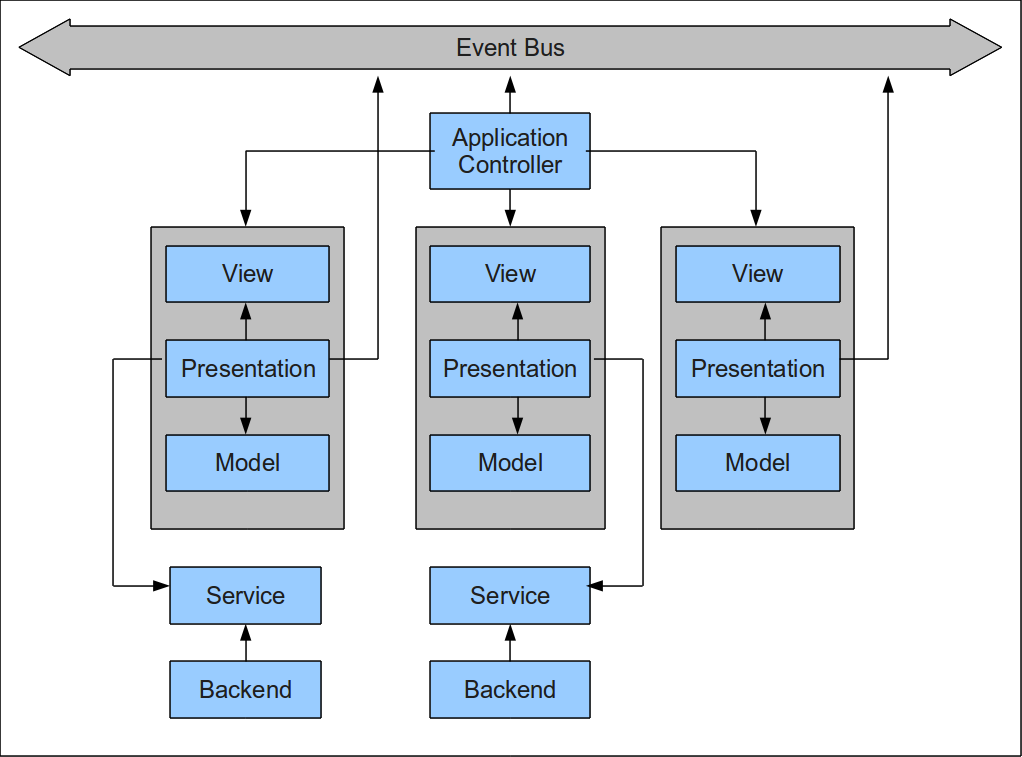
\includegraphics[width=8.5cm]{img/ST/mvp.png}
\caption{Architettura tipica di MVP utilizzando Google Web Toolkit}
\end{figure}

Nel nostro caso questo design pattern sar\`a implementato con il framework MVP con
Activities e Places offerto da GWT 2.1 che semplifica la gestione di alcuni
aspetti consolidati di MVP. In questo framework le Activities svolgono il ruolo
di Presenter e i Places rappresentano gli stati della UI.
\begin{itemize}
  \item{\bo{Activity} }
  \`e l'analogo di presenter in MVP tradizionale. Non contiene alcun componente
  grafico ed il suo avvio e la sua terminazione sono gestite da un
  ActivityManager.
  \item{\bo{Place} }
  un Place in GWT 2.1 rappresenta un particolare stato della UI e viene
  utilizzato anche per tenere una history degli URL che \`e fondamentale per una
  Web Application.

\end{itemize} 
\begin{figure}[h]
\centering
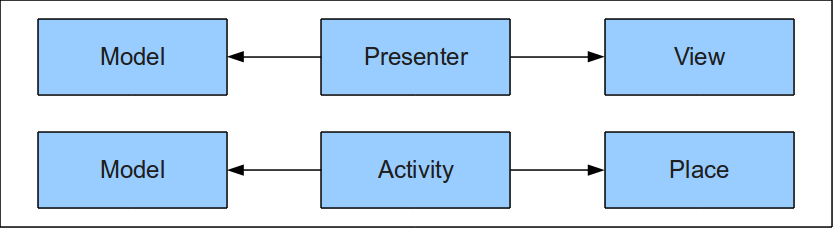
\includegraphics[width=7cm]{img/ST/mvpap.png}
\caption{Comparazione tra MVP tradizionale e MVP con Activities e Places}
\end{figure}

\newpage

\subsubsection{Data Access Object (DAO)  e  Data Transfer Object (DTO)}
\begin{figure}[h]
\centering
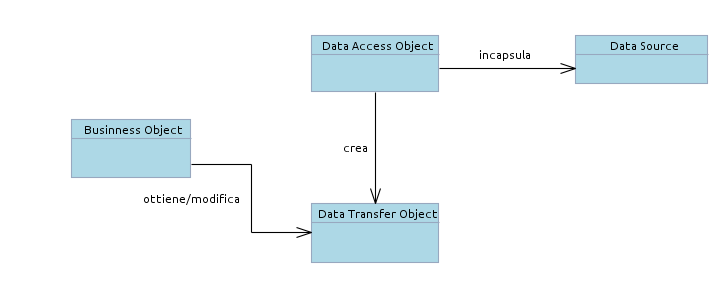
\includegraphics[width=15cm]{img/ST/DAO_DTO.png}
\caption{Diagramma UML delle classi che descrive la struttura dell'utilizzo
simultaneo dei patterns DAO e DTO}
\end{figure}
Questi patterns vengono introdotti all'interno della componente model di MVP e
riguardano gli oggetti utilizzati per l'incapsulamento dei dati nelle
comunicazioni tra client, server e database. 
Il DAO (Data Access Object) \`e un pattern semplice ma fondamentale per
stratificare ed isolare gli accessi al database dalla parte logica
dell'applicazione, nel nostro caso le Activity di MVP. L'implementazione \`e
fondamentalmente una classe che rappresenta un'entit\`a tabellare di un database.
Questi oggetti estratti dal database in alcuni casi possono essere utilizzati
per la comunicazione con i clients ma hanno pesanti restrizioni dovute alla
grande quantit\`a di informazioni e procedure che contengono, per questo motivo
abbiamo deciso di affiancare a DAO anche il pattern Data Transfer Object. Gli
oggetti DTO saranno quelli che verranno scambiati nella comunicazione tra client
e server con il vantaggio di essere pi\`u essenziali dei DAO e la possibilit\`a di
costituire dei pacchetti su misura per la comunicazione. La logica del
tracciamento tra DAO e DTO sar\`a a carico degli oggetti DAO.
\\
Per questo scopo GWT2.1 propone un potente framework per gestire la
comunicazione tra client e server, Request Factory, che implementa i patterns
precedentemente descritti. Abbiamo deciso per\`o di non utilizzarlo, progettando
una nostra implementazione, a causa della documentazione insufficente fornita
da Google.

\newpage
\subsubsection{Abstract factory}
Un abstract factory \`e rappresentata da un'interfaccia che permette di creare dei
prodotti senza specificare classi concrete.

\begin{figure}[h]
\centering
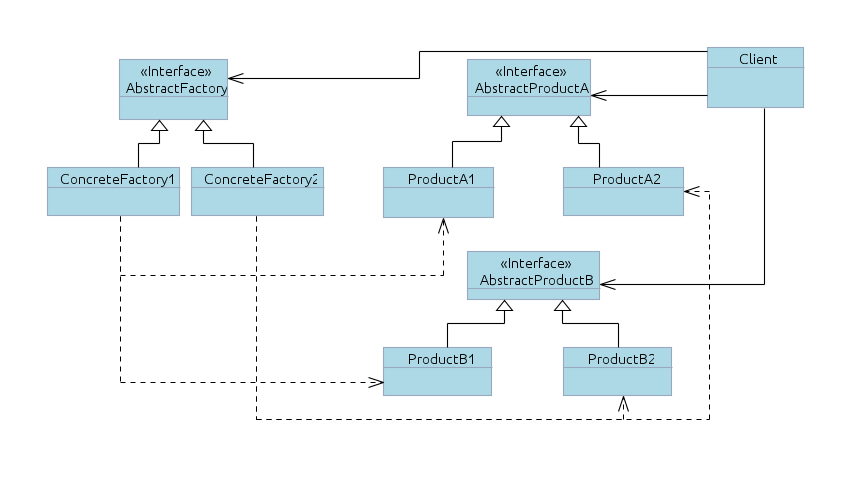
\includegraphics[width=16.5cm]{img/ST/AbstractFactory.png}
\caption{Diagramma UML delle classi che descrive la struttura tradizionale di
Abstract factory}
\end{figure}
Nello specifico lo utilizzeremo per rendere facilmente configurabile il nostro
sistema. L'interfaccia ClientFactory sar\`a utilizzata per ottenere le
intefacce degli elementi architetturali necessari alla nostra applicazione come
ad esempio l'event bus e le varie UI.
Per caricare le differenti implementazioni di ClientFactory a seconda delle
peculiarit\`a dell'utente che vi accede \`e molto conveniente utilizzare il GWT
deferred binding offerto dal toolkit stesso.
Il pattern in questione verr\`a utilizzato per una evidente convenienza in termini
di estendibilit\`a per il futuro anche se allo stadio attuale la factory
implementata sar\`a solamente una.

\newpage
\subsubsection{Singleton}
\begin{figure}[h]
\centering
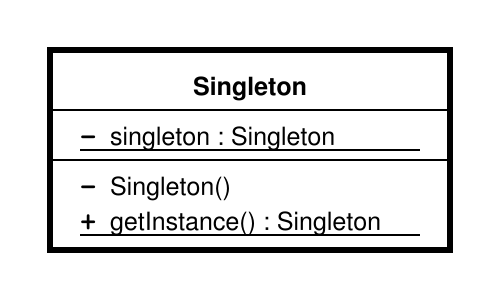
\includegraphics[width=4cm]{img/ST/Singleton.png}
\caption{Diagramma UML delle classi che descrive l'implementazione del design
pattern Singleton}
\end{figure}
Singleton \`e un design pattern creazionale che ha lo scopo di assicurare
l'esistenza di una sola istanza di una certa classe ed avere un punto di accesso
globale a quest'ultima. 
L'implementazione di Singleton diminuisce in generale l'accoppiamento del
sistema.
Utilizzeremo questo pattern per una classe (Persistent manager factory) che si
occupera di creare degli speciali oggetti introdotti da JDO per la
comunicazione con il database (query). \`E molto importante che venga instanziata una sola
istanza di Persistent manager factory e che questa sia visibile all'intero
dell'intero lato server del sistema NetMus. 

\newpage
\subsection{Decomposizione architeturale}
La decomposizione architetturale da noi individuata a partire dalla lista dei
requisiti prodotta dal processo di analisi si compone di tre moduli
fondamentali distribuiti su una parte client e una server. Questi tre moduli, in
accordo con il framework \emph{MVP con Activities e Places} precendetemente
presentato, sono il model che riguarda le parti di businnes logic e businnes
data, la view che contiene l'intera parte grafica del sistema (UI) con i
relativi stati (Places) e il presenter che costituisce il collegamento tra view
e model attraverso le Activities.
\\\\
La struttura sar\`a quindi formata dai seguenti packages:
\begin{figure}[h]
  \centering
  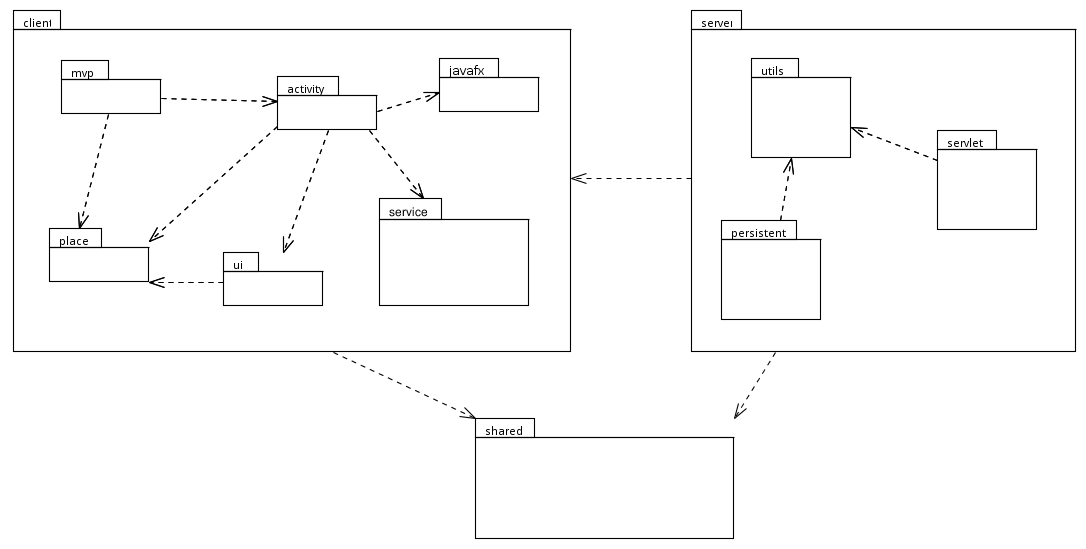
\includegraphics[width=16cm]{img/ST/PackageGeneric.png}
\caption{Diagramma dei package principali di Netmus.}
\end{figure}

\begin{itemize}
  \item Package \emph{client} : definisce la parte client del programma
  \begin {itemize}
    \item Package \emph{client.ui} : comprende l'insieme di viste del sistema,
    rispettando il framework \emph{MVP con Places e Activities}. Ci sar\`a una
    interfaccia per ogni vista, per dare la possibilit\`a di creare in futuro
    pi\`u implementazioni differenti a seconda del dispositivo client;
    \item Package \emph{client.activity} : rappresenta l'insieme di classi
    controllori che formano la logica del sistema. Esse mandano dati aggiornati alle
    viste, gestiscono le richieste delle viste e possono inoltre gestire
    richieste provenienti da altre componenti e mandare eventi propri nell'event-bus;
    \item Package \emph{client.place} : comprende l'insieme di classi Place i
    quali rappresentano un URL associato ad una vista. Gestiscono i parametri
    agganciati all'URL con un Tokenizer interno;
    \item Package \emph{client.mvp} : comprende un ActivityMapper e
    un PlaceHistoryManager che mappano per ogni Place la sua corrispondente
    Activity e gestiscono la cronologia dei Place;
    \item Package \emph{client.service} : rappresenta l'insieme di interfaccie
    che offrono un servizio di comunicazione col server tramite GWT RPC;
    %----------------- TOGLIERE FORSE --------------------
    \item Package \emph{client.applet} : definisce la componente di
    ricezione dei dati estratti dall'Applet precompilata;
    %-------------------------------------------------------
  \end {itemize}
  \item Package \emph{server} : rappresenta la parte server di Netmus;
  \begin{itemize}
    \item Package \emph{server.persistent} : comprende tutte le classi che
    rappresentano un entit\`a JDO (Java Data Object), le quali usate per lo scambio dati tra
    server e Google Datastore;
    \item Package \emph{server.servlet} : comprende tutte le servlet utilizzate
    per interfacciarsi a servizi esterni (es. Google Authentication, YouTube);
    \item Package \emph{server.utils} : comprende classi di utilit\`a per
    svolgere attivit\`a interne al server di varie tipologie;
  \end{itemize}
  \item Package \emph{shared} :  contiene classi condivise tra client e server,
  che verrano anch'esse compilate in JavaScript da GWT, come tutto il package
  client. La maggior parte saranno gli oggetti di trasferimento che
  aderiscono al pattern DTO.
\end{itemize}

\newpage
\subsubsection{Decomposizione architeturale - lato client}
Per soddisfare i requisiti funzionali del sistema NetMus sono state individuate
4 componenti che implementano altrettante UI con la relativa logica di
attivazione delle Activities. Queste sono Login, User, EditProfile e EditSongs
che grazie all'interazione tra le loro parti view, place e activity garantiscono
all'utente tutte le funzionalit\`a attese.\\
Le interfacce Service invece rappresentano il punto di collegamento con il model
la cui implementazione \`e sviluppata principalmente lato server. Queste
interfacce, infatti, vengono accedute dalle Activities poich\'e forniscono tutti i
metodi riguardanti la businness logic. \\\\ 
L'intero schema delle classi individuate durante la progettazione \`e il
sueguente: 
\begin{figure}[h]
  \centering
  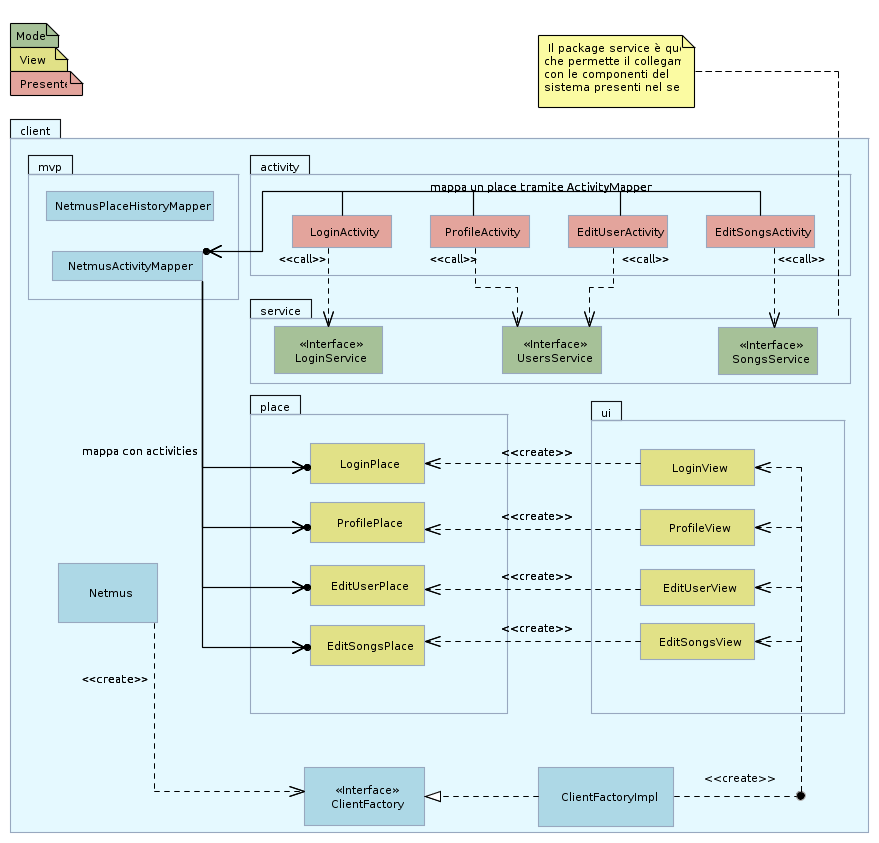
\includegraphics[width=16.5cm]{img/ST/client.png}
\caption{Diagramma delle classi del package client.}
\end{figure}
\newpage
\subsubsection{Decomposizione architeturale - lato server}
Nella parte server si trovano le implementazioni dei Service che hanno
la possibilit\`a di accedere alle informazioni presenti nel database grazie alle
classi DAO presenti nel package \emph{persistent}.
Grande importanza viene data alle classi presenti nel pakage \emph{shared}
poich\'e rendono allo stesso tempo semplice ed efficente il passaggio di
informazioni tra il server e i clients poich\'e incapsulano gli oggetti di
peristenza DAO rimuovendone la parte logica, rispettando il design pattern DTO.
\\\\ L'intero schema delle classi
individuate durante la progettazione \`e il sueguente: \begin{figure}[h]
  \centering
  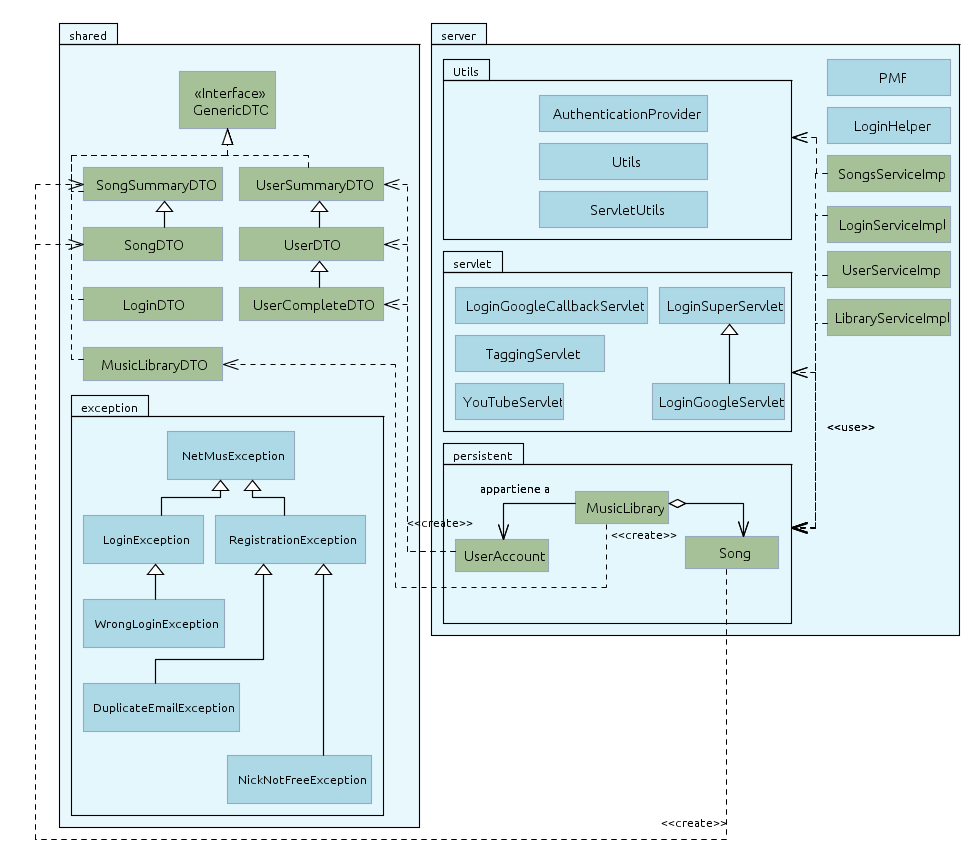
\includegraphics[width=16.5cm]{img/ST/Server&Shared.png}
\caption{Diagramma delle classi dei packages server e shared.}
\end{figure}


\chapter{Descrizione dei singoli componenti}
\section{Package client}
\subsection*{Tipo, obiettivo e funzione del componente} % LASCIARE WARNING
Il package \emph{client} rappresenta la parte del sistema con la quale l'utente
pu\`o interagire. Tutte le sue classi ed i suoi sottopackage saranno compilati in
JavaScript da GWT, prima che il sistema venga depositato nel dominio
\emph{appspot.com} di Google. Contiene la classe \underline{Entry Point}
\co{Netmus}.

\subsection*{Relazioni d'uso di altre componenti}
Il package \emph{client} utilizza i DTO nel package \emph{shared}.

\subsection*{Interfacce con e relazioni d'uso da altre componenti}
Nessuna.

\subsection*{Attivit\`a svolte e dati trattati}
Le attivit\`a svolte dalle sue classi verranno qui di seguito descritte.

\subsection{Classe Netmus}
\subsubsection*{Tipo, obiettivo e funzione del componente}
Questa classe rappresenta l'Entry Point di GWT che genera tutte le altre
componenti e rende disponibile e visibile l'intero sistema.\\
In particolare andr\`a a creare dinamicamente il ClientFactoryImpl adatto, nel
caso ce ne fossero diversi, e lo aggancia insieme all'EventBus al nostro
\co{NetmusPlaceHistoryMapper} ed al \co{NetmusActivityMapper}.
Inoltre allaccia al body Html il widget principale dell'applicazione.

\subsubsection*{Relazioni d'uso di altre componenti}
La classe \co{Netmus} utilizza le classi \co{ClientFactory},
\co{NetmusActivityMapper} e \\\co{NetmusPlaceHistoryMapper}.

\subsubsection*{Interfacce con e relazioni d'uso da altre componenti}
Nessuna.

\subsubsection*{Attivit\`a svolte e dati trattati}
\co{Netmus} praticamente si occupa di avviare il sistema e portare l'utente alla
pagina iniziale di Login o, se gi\`a loggato, alla sua pagina Profilo.

\subsection{Classe ClientFactoryImpl (\emph{Abstract Factory})}
\subsubsection*{Tipo, obiettivo e funzione del componente}
In Netmus \`e disponibile un'unica implementazione dell'intefaccia
ClientFactory, poich\`e per il momento non \`e contemplato un utilizzo di
alternative all'interfaccia utente desktop.
Nella classe si definiscono le propriet\`a di un vista (desktop) del
sistema.

\subsubsection*{Relazioni d'uso di altre componenti}
La classe utilizza \co{EventBus}, \co{PlaceController}, \co{LoginView},
\co{ProfileView}, \co{EditUserView} e
\co{EditSongView}.
\subsubsection*{Interfacce con e relazioni d'uso da altre componenti}
\co{Netmus} crea l'istanza della classe. L'interfaccia \co{ClientFactory} \`e
utilizzata da \co{ActivityMapper} e successivamente dalle \co{Activity} per
l'utilizzo dell'EventBus.
\subsubsection*{Attivit\`a svolte e dati trattati}
La classe si occupa di istanziare l'event bus, il place controller e le varie
view. L'event bus gestisce le comunicazioni tra componenti, il place
controller permette la navigazione tra i Place ed \`e si occupa di avvisare
l'utente prima del passaggio ad uno stato differente.


\newpage
\section{Package client.ui} % LASCIARE WARNING
\subsection*{Tipo, obiettivo e funzione del componente}
Il package \emph{ui} contiene le interfacce e le implementazioni delle View del
sistema. Le View generano gli ambienti grafici con cui gli utenti possono
interagire e si occupano di catturare gli eventi da essi prodotti.

\subsection*{Relazioni d'uso di altre componenti}
Questo package utilizza \emph{place} per creare istanze dei vari Place quando
richiesto.

\subsection*{Interfacce con e relazioni d'uso da altre componenti}
Viene utilizzato dal package \emph{activity}.

\subsection*{Attivit\`a svolte e dati trattati}
In sostanza svolge il compito di organizzare le informazioni del model in un
interfaccia accessibile dall'utente.

\subsection{Classe LoginView}
\subsubsection*{Tipo, obiettivo e funzione del componente}
Il sistema mette a disposizione una vista per l'autenticazione e la
registrazione degli utenti Netmus. La classe \co{LoginViewImpl}
implementa l'interfaccia \co{LoginView} che estende \co{isWidget}
(interfaccia introdotta da GWT 2.1).
\subsubsection*{Relazioni d'uso di altre componenti}
La classe istanzia oggetti di tipo \co{LoginPlace} che definiscono gli stati
attuali della vista.
\subsubsection*{Interfacce con e relazioni d'uso da altre componenti}
La vista viene creata da \co{ClientFactory} ed \`e settata ed utilizzata dalla
\co{LoginActivity}.
\subsubsection*{Attivit\`a svolte e dati trattati}
La classe permette all'utente di scegliere il tipo di registrazione da
effettuare (Google o Netmus), contiene una form per l'inserimento password e
nome utente e pu\`o visualizzare warning se i dati inseriti non sono corretti.

\subsection{Classe ProfileView}
\subsubsection*{Tipo, obiettivo e funzione del componente}
Il sistema mette a disposizione una vista per la visualizzazione dei profili e
dei brani degli altri utenti registrati. La classe \co{ProfileViewImpl}
implementa l'interfaccia \co{ProfileView} che estende \co{isWidget}
(interfaccia introdotta da GWT 2.1).
\subsubsection*{Relazioni d'uso di altrecomponenti} 
La classe istanzia oggetti di tipo \co{ProfilePlace} che definiscono gli stati
attuali della vista.
\subsubsection*{Interfacce con e relazioni d'uso da altre componenti}
 La vista viene creata da \co{ClientFactory} ed \`e settata ed utilizzata dalla
 \co{ProfileActivity}.
 \subsubsection*{Attivit\`a svolte e dati trattati}
Contiene la lista dei profili che l'utente pu\`o visualizzare e gli strumenti
per navigare tra i cataloghi musicali.

\subsection{Classe EditUserView}
\subsubsection*{Tipo, obiettivo e funzione del componente}
Il sistema mette a disposizione una vista per la
modifica delle informazioni personali dell'utente registrato. La classe
\co{EditUserViewImpl} implementa l'interfaccia \co{EditUserView} che estende
\co{isWidget} (interfaccia introdotta da GWT 2.1).

\subsubsection*{Relazioni d'uso di altre componenti}
La classe istanzia oggetti di tipo \co{EditUserPlace} che definiscono gli stati
attuali della vista.
\subsubsection*{Interfacce con e relazioni d'uso da altre componenti}
La vista viene creata da \co{ClientFactory} ed \`e settata ed utilizzata dalla
\co{EditUserActivity}.
\subsubsection*{Attivit\`a svolte e dati trattati}
Mette a disposizione gli strumenti per la modifica delle informazioni personali
dell'utente registrato.

\subsection{Classe EditSongsView}
\subsubsection*{Tipo, obiettivo e funzione del componente}
Il sistema mette a disposizione una vista per visualizzazione e la modifica del
catalogo brani utente. La classe \co{EditSongsViewImpl} implementa l'interfaccia
\co{EditSongsView} che estende \co{isWidget} (interfaccia introdotta da GWT
2.1).
\subsubsection*{Relazioni d'uso di altre componenti}
La classe istanzia oggetti di tipo \co{EditSongsPlace} che definiscono gli stati
attuali della vista.
\subsubsection*{Interfacce con e relazioni d'uso da altre componenti}
La vista viene creata da \co{ClientFactory} ed \`e settata ed utilizzata dalla
\co{EditSongsActivity}.
\subsubsection*{Attivit\`a svolte e dati trattati}
Permette di visualizzare e aggiungere o rimuovere manualmente brani dalla
propria libreria musicale. La rimozione di informazioni non influenza i dati che
Netmus salva sul database.

\newpage
\section{Package client.activity} % LASCIARE WARNING
\subsection*{Tipo, obiettivo e funzione del componente}
Questo package contiene le classi Activity che implementano le funzionalit\`a
usabili da un certo Place. Corrisponde in pratica alla componente Presenter del
pattern MVP originale.
\subsection*{Relazioni d'uso di altre componenti}
Il package usa gli oggetti View di \emph{ui} e Place di \emph{place} per gestire
informazioni di stato o modificatori della vista, ma quando serve pu\`o
utilizzare servizi forniti da \emph{service}.
\subsection*{Interfacce con e relazioni d'uso da altre componenti} 
Le istanze delle classi Activity vengono create dal \co{NetmusActivityMapper}
che quando, riceve una richiesta di una Activity, ritorna una corretta istanza
di tale classe, in base al Place corrente.
\subsection*{Attivit\`a svolte e dati trattati}
Il package \emph{activity} si pu\`o considerare il boss, poich\`e gestisce
l'intera logica di business del client.

\subsection{Classe LoginActivity}
\subsubsection*{Tipo, obiettivo e funzione del componente}
Questa classe sar\`a di tipo \co{AbstractActivity}, implementa il \co{Presenter}
interno alla \co{LoginView} e dovr\`a fornire i servizi destinati ad autenticare
o registrare l'utente.
\subsubsection*{Relazioni d'uso di altre componenti}
Invoca i servizi di autenticazione forniti da \co{LoginService} e utilizza
le relative classi \co{LoginPlace} e \co{LoginView}.
\subsubsection*{Interfacce con e relazioni d'uso da altre componenti} 
Viene creata da \co{NetmusActivityMapper} quando viene richiesta la Activity da
un Place di tipo \co{LoginPlace}.
\subsubsection*{Attivit\`a svolte e dati trattati}
Questa classe gestir\`a, assieme a \co{LoginService}, le richieste di login,
logout, registrazione solo a Netmus, registrazione tramite Google.

\subsection{Classe ProfileActivity}
\subsubsection*{Tipo, obiettivo e funzione del componente}
Questa classe estende \co{AbstractActivity}, implementa il \co{Presenter}
interno alla \co{ProfileView} e fornir\`a i servizi
che il profilo utente dovr\`a offrire all'utente.
\subsubsection*{Relazioni d'uso di altre componenti}
Invoca i servizi di interrogazione e modifica dei dati profilo forniti da
\co{UsersService} e utilizza le relative classi \co{ProfilePlace} e
\co{ProfileView}.
\subsubsection*{Interfacce con e relazioni d'uso da altre componenti}
Viene creata da \co{NetmusActivityMapper} quando viene richiesta la Activity da
un Place di tipo \co{ProfilePlace}.
\subsubsection*{Attivit\`a svolte e dati trattati}
Questa classe gestisce, assieme a \co{UsersService}, le attivit\`a utili alla
creazione ed interazione con l'utente della pagina principale come: la
richiesta dei dati utente dettagliati, della lista dei brani, del dettaglio di
un brano, ecc.

\subsection{Classe EditUserActivity}
\subsubsection*{Tipo, obiettivo e funzione del componente}
Questa classe estende \co{AbstractActivity}, implementa il \co{Presenter}
interno alla \co{EditUserView} e fornisce i servizi per la modifica dei dati
personali.
\subsubsection*{Relazioni d'uso di altre componenti}
Invoca i servizi di interrogazione e modifica dei dati profilo forniti da
\co{UsersService} e utilizza le relative classi \co{EditUserPlace} e
\co{EditUserView}.
\subsubsection*{Interfacce con e relazioni d'uso da altre componenti}
Viene creata da \co{NetmusActivityMapper} quando viene richiesta la Activity da
un Place di tipo \co{EditUserPlace}.
\subsubsection*{Attivit\`a svolte e dati trattati}
Questa classe gestisce, assieme a \co{UsersService}, le attivit\`a utili alla
modifica delle informazioni personali visualizzate nel profilo.

\subsection{Classe EditSongsActivity}
\subsubsection*{Tipo, obiettivo e funzione del componente}
Questa classe estende \co{AbstractActivity}, implementa il \co{Presenter}
interno alla \co{EditSongsView} e fornisce i servizi per la visualizzazione e la
modifica della libreria musicale.
\subsubsection*{Relazioni d'uso di altre componenti} Invoca i servizi di
interrogazione e modifica dei dati musicali forniti da \co{SongsService} e
utilizza le relative classi \co{EditSongsPlace} e \co{EditSongsView}.
\subsubsection*{Interfacce con e relazioni d'uso da altre componenti}
Viene creata da \co{NetmusActivityMapper} quando viene richiesta la Activity da
un Place di tipo \co{EditSongsPlace}.
\subsubsection*{Attivit\`a svolte e dati trattati}
Questa classe gestisce, assieme a \co{songsService}, le attivit\`a utili alla
visualizzazione e modifica della libreria musicale personale.

\newpage
\section{Package client.place} % LASCIARE WARNING
\subsection*{Tipo, obiettivo e funzione del componente}
Il package contiene le classi di tipo Place. I Place sono indispensabili
per far s\`i che la corrispondente Activity sia accessibile via URL.
\subsection*{Relazioni d'uso di altre componenti}
A questo package appartengono le classi \co{LoginPlace}, \co{ProfilePlace},
\co{EditUserPlace}, \\\co{EditSongsPlace}.
\subsection*{Interfacce con e relazioni d'uso da altre componenti}
 I suoi elementi vengono utilizzati dal package \emph{mvp}.
\subsection*{Attivit\`a svolte e dati trattati}
Organizza i Places.

\subsection{Classe LoginPlace}
\subsubsection*{Tipo, obiettivo e funzione del componente}
\co{LoginPlace} estende la classe \co{Place} messa a disposizione da GWT. La
classe \`e associata alla classe interna \co{Tokenizer} che permette di
serializzare lo stato del Place in un simbolo (token) URL.
\subsubsection*{Relazioni d'uso di altre componenti}
Nessuna.
\subsubsection*{Interfacce con e relazioni d'uso da altre componenti}
La classe \`e creata da \co{LoginView} utilizzata da \co{LoginActivity}.
\subsubsection*{Attivit\`a svolte e dati trattati}
Il compito della classe \`e quello di indicizzare gli stati di
\co{LoginActivity} in modo da rendere accessibili le funzionalit\`a di history e
bookmarking del browser.

\subsection{Classe ProfilePlace}
\subsubsection*{Tipo, obiettivo e funzione del componente}
\co{ProfilePlace} estende la classe \co{Place} messa a disposizione da GWT. La
classe \`e associata alla classe interna \co{Tokenizer} che permette di
serializzare lo stato del Place in un simbolo (token) URL.
\subsubsection*{Relazioni d'uso di altre componenti}
Nessuna.
\subsubsection*{Interfacce con e relazioni d'uso da altre componenti}
La classe \`e creata da \co{ProfileView} utilizzata da \co{ProfileActivity}.
\subsubsection*{Attivit\`a svolte e dati trattati}
Il compito della classe \`e quello di indicizzare gli stati di
\co{ProfileActivity} in modo da rendere accessibili le funzionalit\`a di history
e bookmarking del browser.

\subsection{Classe EditUserPlace}
\subsubsection*{Tipo, obiettivo e funzione del componente}
\co{EditUserPlace} estende la classe \co{Place} messa a disposizione da GWT. La
classe \`e associata alla classe interna \co{Tokenizer} che permette di
serializzare lo stato del Place in un simbolo (token) URL.
\subsubsection*{Relazioni d'uso di altre componenti}
Nessuna.
\subsubsection*{Interfacce con e relazioni d'uso da altre componenti}
La classe \`e creata da \co{EditUserView} utilizzata da \co{EditUserActivity}.
\subsubsection*{Attivit\`a svolte e dati trattati}
Il compito della classe \`e quello di indicizzare gli stati di
\co{EditUserActivity} in modo da rendere accessibili le funzionalit\`a di
history e bookmarking del browser.

\subsection{Classe EditSongsPlace}
\subsubsection*{Tipo, obiettivo e funzione del componente}
\co{EditSongsPlace} estende la classe \co{Place} messa a disposizione da GWT. La
classe \`e associata alla classe interna \co{Tokenizer} che permette di
serializzare lo stato del Place in un simbolo (token) URL.
\subsubsection*{Relazioni d'uso di altre componenti}
Nessuna.
\subsubsection*{Interfacce con e relazioni d'uso da altre componenti}
La classe \`e creata da \co{EditSongsView} utilizzata da \co{EditSongsActivity}.
\subsubsection*{Attivit\`a svolte e dati trattati}
Il compito della classe \`e quello di indicizzare gli stati di
\co{EditSongsActivity} in modo da rendere accessibili le funzionalit\`a di
history e bookmarking del browser.

\newpage
\section{Package client.mvp} % LASCIARE WARNING
\subsection*{Tipo, obiettivo e funzione del componente}
Il package contiene le classi funzionali al meccanismo delle Activity e dei
Places.
\subsection*{Relazioni d'uso di altre componenti}
Fanno parte di questo package le classi \co{NetmusHistoryMapper} e
\co{NetmusActivityMapper}.
\subsection*{Interfacce con e relazioni d'uso da altre componenti}
Nessuna.
\subsection*{Attivit\`a svolte e dati trattati}
Le attivit\`a svolte dalle sue classi verranno qui di seguito descritte.

\subsection{Classe NetmusActivityMapper}
\subsubsection*{Tipo, obiettivo e funzione del componente}
Questa classe si occupa di mappare ogni attivita con il corrispondente Place.
\subsubsection*{Relazioni d'uso di altre componenti}
La classe utilizza istanze di classi appartenenti al package
\emph{client.place} e crea istanze di classi appartenenti al package
\emph{client.activity}.
\subsubsection*{Interfacce con e relazioni d'uso da altre
componenti} Nessuna
\subsubsection*{Attivit\`a svolte e dati trattati}
Tramite un riferimento ad un Place crea e restituisce un oggetto activity.

\subsection{Classe NetmusPlaceHistoryMapper}
\subsubsection*{Tipo, obiettivo e funzione del componente}
Dichiara e riferisce tutti i places che saranno utilizzati da Netmus.
\subsubsection*{Relazioni d'uso di altre componenti}
Utilizza i PlaceTokenizer
\subsubsection*{Interfacce con e relazioni d'uso da altre componenti}
Il PlaceHistoryHandler utilizza la classe per la sincronizzazione del URL.
\subsubsection*{Attivit\`a svolte e dati trattati}
Funge da connessione tra i PlaceTokenizer (classe interna ad ogni Place) e il
PlaceHistoryHandler (messo a disposizione da GWT) che sincronizza l'URL del
browser con i vari Place.

\newpage
\section{Package client.service} % LASCIARE WARNING
\subsection*{Tipo, obiettivo e funzione del componente}
Il package \co{service} \`e costituito da tutte le interfacce dei servizi remoti
offerti dal server. Le funzionalit\`a delle classi in esso contenute saranno
divise in base al tipo di servizio offerto.  Per ognuno di questi sar\`a
presente un'interfaccia normale (che estende \co{RemoteService}) e un
interfaccia \bo{asincrona}.

\subsection*{Relazioni d'uso di altre componenti}
Queste interfacce vengono implementate su \emph{server}, perci\`o non
hanno relazioni d'uso definite. Verranno sempre usati oggetti DTO (definiti in
\emph{shared}) come pacchetti di scambio nei servizi tra \emph{client} e
\emph{server}.

\subsection*{Interfacce con e relazioni d'uso da altre componenti}
Verranno istanziati degli oggetti di \emph{service} col metodo del
\emph{deferred binding} dalla classe di Entry Point \co{Netmus}, pur avendo
visibilit\`a solamente delle interfacce. Verranno poi usati dalle varie Activity.

\subsection*{Attivit\`a svolte e dati trattati}
Vengono forniti tutti i servizi che il server sar\`a in grado di dare, i dati
trattati saranno i DTO definiti nel package \emph{shared}.

\subsection{Interfaccia SongsService (e SongServiceAsync)}
\subsubsection*{Tipo, obiettivo e funzione del componente}
Questa classe dovr\`a consentire alle componenti Activity di \emph{client} di
inviare richieste di vario tipo a \emph{server} riguardanti informazioni sui
brani musicali. Sar\`a presente anche \co{SongServiceAsync}, che gestir\`a il ritorno
dai metodi in maniera asincrona.

\subsubsection*{Relazioni d'uso di altre componenti}
Queste interfacce verranno implementate su \emph{server}, perci\`o non
avranno relazioni d'uso definite, se non con gli oggetti DTO
(\co{UserDTO, SongDTO}, \co{SongSummaryDTO}, \co{MusicLibraryDTO}) che verranno
utilizzati per il trasferimento client-server.

\subsubsection*{Interfacce con e relazioni d'uso da altre componenti}
Questa interfaccia verr\`a istanziata da \co{Netmus} tramite deferred
binding e verr\`a utilizzata da \co{ProfileActivity} ed \co{EditSongsActivity}.

\subsubsection*{Attivit\`a svolte e dati trattati}
Questa interfaccia fornir\`a l'accesso a servizi per richiedere qualsiasi tipo
di informazione riguardante i brani musicali e utilizzer\`a dati di tipo SongDTO
e SongSummaryDTO.

\subsection{Interfaccia UsersService (e UsersServiceAsync)}
\subsubsection*{Tipo, obiettivo e funzione del componente}
Questa classe consentir\`a alle componenti Activity di \emph{client} di inviare
richieste di vario tipo a \emph{server} riguardanti le informazioni personali
dell'utente da mostrare  nell'interfaccia grafica. Sar\`a presente anche
\co{UsersServiceAsync}, che gestir\`a il ritorno dai metodi in maniera asincrona.

\subsubsection*{Relazioni d'uso di altre componenti}
Queste interfacce verranno implementate su \emph{server}, perci\`o non
avranno relazioni d'uso definite, se non con gli oggetti DTO (\co{UserDTO},
\co{UserSummaryDTO}, \co{UserCompleteDTO}) che verranno utilizzati per il
trasferimento client-server.

\subsubsection*{Interfacce con e relazioni d'uso da altre componenti}
Questa interfaccia verr\`a istanziata da \co{Netmus} tramite deferred
binding e verr\`a utilizzata da \co{EditUserActivity} e \co{ProfileActivity}.

\subsubsection*{Attivit\`a svolte e dati trattati}
Questa interfaccia fornir\`a l'accesso a servizi per richiedere qualsiasi tipo
di informazione riguardante gli utenti del sistema e utilizzer\`a dati di tipo
\co{UserDTO}, \co{UserSummaryDTO} e\\\co{UserCompleteDTO}.

\subsection{Interfaccia LoginService (e LoginServiceAsync)}
\subsubsection*{Tipo, obiettivo e funzione del componente}
Questa classe consentir\`a alle componenti Activity di \emph{client} di inviare
richieste di vario tipo a \emph{server} riguardanti la fase di autenticazione e
logout degli utenti. Sar\`a presente anche \co{LoginServiceAsync}, che gestir\`a
il ritorno dai metodi in maniera asincrona.

\subsubsection*{Relazioni d'uso di altre componenti}
Queste interfacce verranno implementate su \emph{server}, perci\`o non
avranno relazioni d'uso definite, se non con oggetti \co{LoginDTO} che
vengono utilizzati per il trasferimento client-server.

\subsubsection*{Interfacce con e relazioni d'uso da altre componenti}
Questa interfaccia verr\`a istanziata da \co{Netmus} tramite deferred
binding e verr\`a utilizzata \\\co{LoginActivity} e dalle altre Activity che
permetterano il logout dell'utente.

\subsubsection*{Attivit\`a svolte e dati trattati}
Questa interfaccia fornir\`a l'accesso a servizi per richiedere qualsiasi tipo
di informazione riguardante gli utenti del sistema e utilizzer\`a dati di tipo
\co{UserDTO}, \co{UserSummaryDTO} e \bo{UserCompleteDTO}.


%--------------- FORSE -------------------------------
\section{Package client.applet} % LASCIARE WARNING
\subsection*{Obiettivo e funzione del componente}
Questo package conterr\`a le classi necessarie a gestire richieste e segnali
provenienti dalla applet precompilata, che andremo ad inserire nel programma.
Tale applet avr\`a la funzione di effettuare la scansione e l'estrazione
automatica dei tag dei file musicali Mp3, presenti nei dispositivi di
archiviavione di massa che vengono collegati alla macchina dell'utente.\\
Per comunicare con tale applet sono state valutate due possibili metodologie
d'implementazione: l'uso di una libreria che crea un sistema proxy tra la applet
e GWT; oppure l'utilizzo di \underline{JSNI} (JavaScript Native Interface) che
sostanzialmente ci permetterebbe di fare chiamate da JavaScript al codice Java e
vice versa.

\subsection*{Meccanismo di lavoro del componente}
Una volta ricevuta una richiesta da parte della applet, verr\`a gestita da un
Service che si occuper\`a di elaborare i dati col supporto del server, per poi
notificare all'utente l'avvenuta estrazione, e fargliela valutare e accettare.
Una volta accettata la lista brani, si richiede la memorizzazione nel DataStore
tramite \co{SongsService}.

%------------------------------------------------------

\newpage
\section{Package server}
\begin{figure}[h]
  \centering
  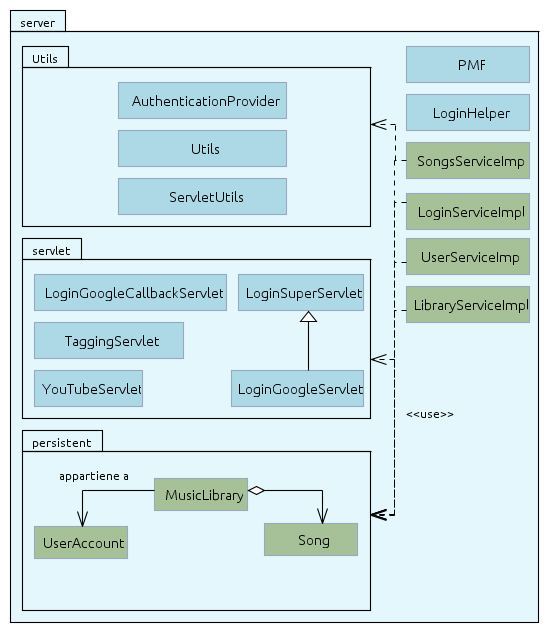
\includegraphics[width=10cm]{img/ST/Server.png}
\caption{Diagramma delle classi del package server.}
\end{figure}

\subsection*{Tipo, obiettivo e funzione del componente} % LASCIARE WARNING
Questo package racchiude tutte le classi che collaborano al fine di gestire la
business logic del sistema, ovvero tutte quelle operazioni che potranno essere
compiute sui dati raccolti. Contiene inoltre delle classi di interfacciamento
con il DataStore stesso che consentono il controllo sulla persistenza dei dati.

\subsection*{Relazioni d'uso di altre componenti}
Si fa utilizzo delle classi presenti nel package \emph{shared} in cui vengono
incapsulati tutti i dati in uscita del server.

\subsection*{Interfacce con e relazioni d'uso da altre componenti}
Il package \emph{server} si interfaccia direttamente con \emph{shared} e tramite
questo e con la presenza del package \emph{service} si interfaccia anche con
\emph{client}.

\subsection*{Attivit\`a svolte e dati trattati}
Le attivit\`a svolte dalle sue classi verranno qui di seguito descritte.

\subsection{Classe SongsServiceImpl}
\subsubsection*{Tipo, obiettivo e funzione del componente}
Questa classe corrisponde all'implementazione del \co{SongsService} (di
\emph{client}) ed estende la classe \co{RemoteServiceServlet}.

\subsubsection*{Relazioni d'uso di altre componenti}
Oltre ad utilizzare ovviamente i DTO in \emph{shared}, verranno creati,
immagazzinati oppure usati i relativi oggetti \emph{persistent}.
Potranno essere usati opportuni servizi in \emph{servlet} per andare a prelevare
informazioni sui brani da servizi esterni oppure per cercare il corrispettivo
link di streming audio-video (tipo YouTube).

\subsubsection*{Interfacce con e relazioni d'uso da altre componenti}
Viene usata dal \emph{client} che ne genera un istanza tramite deferred binding,
utilizzando l'interfaccia \co{SongsService}.

\subsubsection*{Attivit\`a svolte e dati trattati}
Descritte nell'interfaccia lato \emph{client}.

\subsection{Classe UsersServiceImpl}
\subsubsection*{Tipo, obiettivo e funzione del componente}
Questa classe corrisponde all'implementazione del \co{UsersService} (di
\emph{client}) ed estende la classe \co{RemoteServiceServlet}.

\subsubsection*{Relazioni d'uso di altre componenti}
Oltre ad utilizzare ovviamente i DTO in \emph{shared}, verranno creati,
immagazzinati oppure usati i relativi oggetti \emph{persistent}.

\subsubsection*{Interfacce con e relazioni d'uso da altre componenti}
Viene usata dal \emph{client} che ne genera un istanza tramite deferred binding,
utilizzando l'interfaccia \co{UsersService}.

\subsubsection*{Attivit\`a svolte e dati trattati}
Descritte nell'interfaccia lato \emph{client}.

\subsection{Classe LoginServiceImpl}
\subsubsection*{Tipo, obiettivo e funzione del componente}
Questa classe corrisponde all'implementazione del \co{LoginService} (di
\emph{client}) ed estende la classe \co{RemoteServiceServlet}.

\subsubsection*{Relazioni d'uso di altre componenti}
Utilizzar\`a i DTO in \emph{shared} e utilizzer\`a le \co{HttpSession} per
gestire le sessioni dell'utente e dargli o meno i diritti d'accesso.
Verranno utilizzate funzionalit\`a interne di gestione login definite in
\co{LoginHelper}. Potranno essere usate opportune classi in \emph{servlet} per
andare ad utilizzare servizi di login e reperimento informazioni utente esterni
(Google Account).

\subsubsection*{Interfacce con e relazioni d'uso da altre componenti}
Viene usata dal \emph{client} che ne genera un istanza tramite deferred binding,
utilizzando l'interfaccia \co{LoginService}.

\subsubsection*{Attivit\`a svolte e dati trattati}
Descritte nell'interfaccia lato \emph{client}.

\subsection{Classe LoginHelper}
\subsubsection*{Tipo, obiettivo e funzione del componente}
La classe \co{LoginHelper} \`e stata pensata per offrire funzionalit\`a statiche
per gestire le sessioni HTML, utili a \co{LoginServiceImpl} ed a \emph{servlet}.

\subsubsection*{Relazioni d'uso di altre componenti}
User\`a al suo interno le classi di utilit\`a per i servlet definite in
\emph{utils} e l'oggetto di persistenza \co{UserAccount}.

\subsubsection*{Interfacce con e relazioni d'uso da altre componenti}
Questa classe viene utilizzat\`a da \co{LoginServiceImpl} e nel package
\emph{servlet} dalle classi dedicate al Login.

\subsubsection*{Attivit\`a svolte e dati trattati}
Le funzionali\`a che metter\`a a disposizione sono quelle di individuare se
l'utente corrente \`e gi\`a loggato o meno, e di riprendere la
sessione restituendo un \emph{persistent} \co{UserAccount} nel caso esso sia
gi\`a loggato.

\subsection{Classe PMF (Singleton)}
\subsubsection*{Tipo, obiettivo e funzione del componente}
\co{PMF} \`e una classe final che segue il pattern Singleton, illustrato
nell'introduzione. Ha la funzione di creare un'unica istanza del
\co{PersistentManagerFactory} (\emph{javax.jdo})e di restituirla a qualunque
oggetto la richieda. Quest'ultimo da la possibilit\`a di interagire con il DataStore, inviando
query, memorizzando oggetti \emph{persistent} o richiedendo liste di oggetti
tramite semplici metodi.

\subsubsection*{Relazioni d'uso di altre componenti}
Vengono usate le classi di \emph{javax.jdo} \co{PersistentManager},
\co{PersistentManagerFactory}\\ e \co{JDOHelper}.

\subsubsection*{Interfacce con e relazioni d'uso da altre componenti}
Questa classe pu\`o essere utilizzata da qualunque classe di \emph{server}, ogni
qualvolta ci sia bisogno di avere il \co{PersistentManager} per interagire col
DataStore.

\subsubsection*{Attivit\`a svolte e dati trattati}
Crea un'unica istanza del \co{PersistentManagerFactory} e tramite un metodo
statico \emph{get()} la passa alle classi, in maniera da dargli la possibilit\`a
di usare il database.


\section{Package server.peristent} % LASCIARE WARNING
\subsection*{Tipo, obiettivo e funzione del componente}
\subsection*{Relazioni d'uso di altre componenti}
\subsection*{Interfacce con e relazioni d'uso da altre componenti}
\subsection*{Attivit\`a svolte e dati trattati}

\subsection{Classe UserAccount}
\subsubsection*{Tipo, obiettivo e funzione del componente}
\subsubsection*{Relazioni d'uso di altre componenti}
\subsubsection*{Interfacce con e relazioni d'uso da altre componenti}
\subsubsection*{Attivit\`a svolte e dati trattati}

\subsection{Classe MusicLibrary}
\subsubsection*{Tipo, obiettivo e funzione del componente}
\subsubsection*{Relazioni d'uso di altre componenti}
\subsubsection*{Interfacce con e relazioni d'uso da altre componenti}
\subsubsection*{Attivit\`a svolte e dati trattati}

\subsection{Classe Song}
\subsubsection*{Tipo, obiettivo e funzione del componente}
\subsubsection*{Relazioni d'uso di altre componenti}
\subsubsection*{Interfacce con e relazioni d'uso da altre componenti}
\subsubsection*{Attivit\`a svolte e dati trattati}

\newpage
\section{Package server.servlet} % LASCIARE WARNING
\subsection*{Tipo, obiettivo e funzione del componente}
\subsection*{Relazioni d'uso di altre componenti}
\subsection*{Interfacce con e relazioni d'uso da altre componenti}
\subsection*{Attivit\`a svolte e dati trattati}

\subsection{Classe LoginSuperServlet}
\subsubsection*{Tipo, obiettivo e funzione del componente}
\subsubsection*{Relazioni d'uso di altre componenti}
\subsubsection*{Interfacce con e relazioni d'uso da altre componenti}
\subsubsection*{Attivit\`a svolte e dati trattati}

\subsection{Classe LoginGoogleServlet}
\subsubsection*{Tipo, obiettivo e funzione del componente}
\subsubsection*{Relazioni d'uso di altre componenti}
\subsubsection*{Interfacce con e relazioni d'uso da altre componenti}
\subsubsection*{Attivit\`a svolte e dati trattati}

\subsection{Classe LoginGoogleCallbackServlet}
\subsubsection*{Tipo, obiettivo e funzione del componente}
\subsubsection*{Relazioni d'uso di altre componenti}
\subsubsection*{Interfacce con e relazioni d'uso da altre componenti}
\subsubsection*{Attivit\`a svolte e dati trattati}

\subsection{Classe YouTubeServlet (da decidere tipo di servlet)}
\subsubsection*{Tipo, obiettivo e funzione del componente}
\subsubsection*{Relazioni d'uso di altre componenti}
\subsubsection*{Interfacce con e relazioni d'uso da altre componenti}
\subsubsection*{Attivit\`a svolte e dati trattati}

\newpage
\subsection{Classe TaggingServlet(da decidere . . .)}
\subsubsection*{Tipo, obiettivo e funzione del componente}
\subsubsection*{Relazioni d'uso di altre componenti}
\subsubsection*{Interfacce con e relazioni d'uso da altre componenti}
\subsubsection*{Attivit\`a svolte e dati trattati}

\section{Package server.utils} % LASCIARE WARNING
\subsection*{Tipo, obiettivo e funzione del componente}
\subsection*{Relazioni d'uso di altre componenti}
\subsection*{Interfacce con e relazioni d'uso da altre componenti}
\subsection*{Attivit\`a svolte e dati trattati}

\subsection{Classe AuthenticationProvider}
\subsubsection*{Tipo, obiettivo e funzione del componente}
\subsubsection*{Relazioni d'uso di altre componenti}
\subsubsection*{Interfacce con e relazioni d'uso da altre componenti}
\subsubsection*{Attivit\`a svolte e dati trattati}

\subsection{Classe ServletUtils}
\subsubsection*{Tipo, obiettivo e funzione del componente}
\subsubsection*{Relazioni d'uso di altre componenti}
\subsubsection*{Interfacce con e relazioni d'uso da altre componenti}
\subsubsection*{Attivit\`a svolte e dati trattati}

\subsection{Classe Utils}
\subsubsection*{Tipo, obiettivo e funzione del componente}
\subsubsection*{Relazioni d'uso di altre componenti}
\subsubsection*{Interfacce con e relazioni d'uso da altre componenti}
\subsubsection*{Attivit\`a svolte e dati trattati}

\newpage
\section{Package shared} % LASCIARE WARNING
\begin{figure}[h]
  \centering
  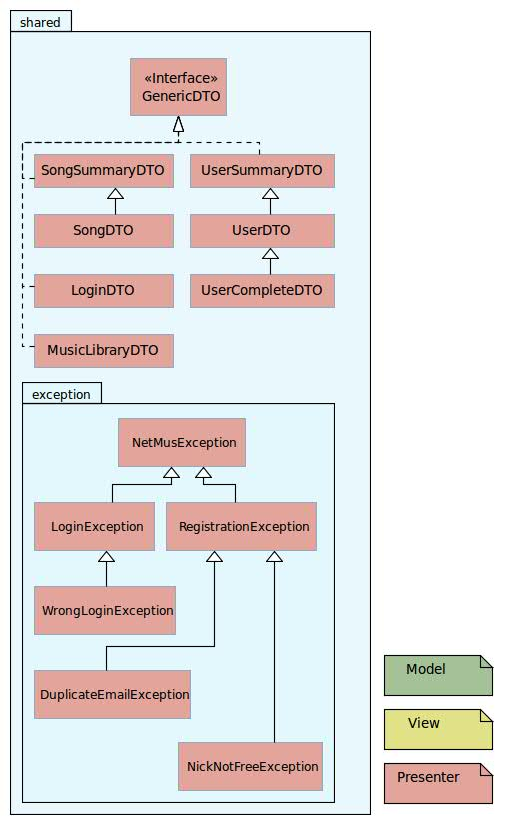
\includegraphics[width=7cm]{img/ST/Shared.png}
\caption{Diagramma delle classi del package shared.}
\end{figure}
\subsection*{Tipo, obiettivo e funzione del componente}
Il package \textit{shared} contiene le classi degli oggetti che vengono
scambiati tra client e server; in particolare, troviamo presenti le classi che
aderiscono al pattern DTO.
\subsection*{Relazioni d'uso di altre componenti}
Tutte le classi di questo package implementano l'interfaccia
\textit{java.io.Serializable} per poter essere serializzate e quindi inviate
attraverso la rete. 
\subsection*{Interfacce con e relazioni d'uso da altre componenti}
Viene utilizzata dalle classi dei package \textit{client} e \textit{server} per
lo scambio di dati e/o informazioni.
\subsection*{Attivit\`a svolte e dati trattati}
In generale, le classi di questo package si occupano di inglobare e trasportare
le informazioni attraverso la rete, per le comunicazioni tra server e client.
Vengono qui di seguito descritte pi\`u in dettaglio.

\subsection{Interfaccia GenericDTO}
\subsubsection*{Tipo, obiettivo e funzione del componente}
Interfaccia comune per le classi DTO. Definisce una generica classe che potr\`a
essere usata come contenitore dei dati di una DAO.
\subsubsection*{Relazioni d'uso di altre componenti}
Vedere la descrizione del package.
\subsubsection*{Interfacce con e relazioni d'uso da altre componenti}
Viene implementata dalle classi del package \textit{shared}.
\subsubsection*{Attivit\`a svolte e dati trattati}
Nessuna. 

\subsection{Classe UserSummaryDTO}
\subsubsection*{Tipo, obiettivo e funzione del componente}
Contiene e rappresenta i dati pi\`u comunemente utilizzati di un utente, ovvero
quelli che vengono visualizzati in un profilo.
\subsubsection*{Relazioni d'uso di altre componenti}
Implementa l'interfaccia \textit{GenericDTO}.
\subsubsection*{Interfacce con e relazioni d'uso da altre componenti}
Vedere la descrizione del package.
\subsubsection*{Attivit\`a svolte e dati trattati}
Funge da contenitore per i dati pi\`u comunemente utilizzati dell'utente, come
per esempio nick ed email.

\subsection{Classe UserDTO}
\subsubsection*{Tipo, obiettivo e funzione del componente}
Contiene e rappresenta la maggior parte dei dati di un utente, pi\`u
precisamente quelli richiesti alla registrazione.
\subsubsection*{Relazioni d'uso di altre componenti}
Estende la classe \textit{UserSummaryDTO}.
\subsubsection*{Interfacce con e relazioni d'uso da altre componenti}
Vedere la descrizione del package.
\subsubsection*{Attivit\`a svolte e dati trattati}
Funge da contenitore per i dati dettagliati di un utente.

\subsection{Classe UserCompleteDTO}
\subsubsection*{Tipo, obiettivo e funzione del componente}
Contiene e rappresenta tutti i dati di un utente, a partire da quelli
visualizzati sul profilo, a quelli interni del sistema.
\subsubsection*{Relazioni d'uso di altre componenti}
Estende la classe \textit{UserDTO}.
\subsubsection*{Interfacce con e relazioni d'uso da altre componenti}
Vedere la descrizione del package.
\subsubsection*{Attivit\`a svolte e dati trattati}
Funge da contenitore per tutti dati dell'utente, dal nick al numero di
registrazione.

\subsection{Classe SongSummaryDTO}
\subsubsection*{Tipo, obiettivo e funzione del componente}
Contiene e rappresenta i dati pi� comunemente utilizzati di un brano, ovvero
quelli che vengono visualizzati in una playlist all'interno di un profilo.
\subsubsection*{Relazioni d'uso di altre componenti}
Implementa l'interfaccia \textit{GenericDTO}.
\subsubsection*{Interfacce con e relazioni d'uso da altre componenti}
Vedere la descrizione del package.
\subsubsection*{Attivit\`a svolte e dati trattati}
Funge da contenitore per i dati pi\`u comunemente utilizzati di un brano, come
per esempio titolo ed autore.

\subsection{Classe SongDTO}
\subsubsection*{Tipo, obiettivo e funzione del componente}
Contiene e rappresenta tutti i dati di un brano, compresi quelli interni del
sistema. 
\subsubsection*{Relazioni d'uso di altre componenti}
Estende la classe \textit{SongSummaryDTO}.
\subsubsection*{Interfacce con e relazioni d'uso da altre componenti}
Vedere la descrizione del package.
\subsubsection*{Attivit\`a svolte e dati trattati}
Funge da contenitore per tutti dati del brano, dal titolo al numero
identificativo del brano. 

\subsection{Classe LoginDTO}
\subsubsection*{Tipo, obiettivo e funzione del componente}
Contiene e rappresenta i dati di login di un utente.
\subsubsection*{Relazioni d'uso di altre componenti}
Implementa l'interfaccia \textit{GenericDTO}.
\subsubsection*{Interfacce con e relazioni d'uso da altre componenti}
Vedere la descrizione del package.
\subsubsection*{Attivit\`a svolte e dati trattati}
Trasporta nome utente e passwsord dal client al server per l'autenticazione.

\subsection{Classe MusicLibraryDTO}
\subsubsection*{Tipo, obiettivo e funzione del componente}
\subsubsection*{Relazioni d'uso di altre componenti}
\subsubsection*{Interfacce con e relazioni d'uso da altre componenti}
\subsubsection*{Attivit\`a svolte e dati trattati}

\subsection{Classe NetMusException}
\subsubsection*{Tipo, obiettivo e funzione del componente}
Generica eccezione del nostro programma.
\subsubsection*{Relazioni d'uso di altre componenti}
Estende la classe \textit{Exception}
\subsubsection*{Interfacce con altre componenti}
Vedere la descrizione del package.
\subsubsection*{Attivit\`a svolte e dati trattati}
Rappresenta una generica eccezione usata all'interno del sistema NetMus.
Tutte le altre eccezioni estendono questa.

\subsection{Classe LoginException}
\subsubsection*{Tipo, obiettivo e funzione del componente}
Indica un generico errore rilevato durante il tentativo di login.
\subsubsection*{Relazioni d'uso di altre componenti}
Estende la classe \textit{NetMusException}
\subsubsection*{Interfacce con altre componenti}
Vedere la descrizione del package.
\subsubsection*{Attivit\`a svolte e dati trattati}
Nessuna.

\subsection{Classe WrongLoginException}
\subsubsection*{Tipo, obiettivo e funzione del componente}
Indica dei dati errati di login.
\subsubsection*{Relazioni d'uso di altre componenti}
Estende la classe \textit{LoginException}
\subsubsection*{Interfacce con altre componenti}
Vedere la descrizione del package.
\subsubsection*{Attivit\`a svolte e dati trattati}
Indica che username e/o password sono errati.

\subsection{Classe RegistrationException}
\subsubsection*{Tipo, obiettivo e funzione del componente}
Indica un generico errore rilevato durante la registrazione di un nuovo utente.
\subsubsection*{Relazioni d'uso di altre componenti}
Estende la classe \textit{NetMusException}
\subsubsection*{Interfacce con altre componenti}
Vedere la descrizione del package.
\subsubsection*{Attivit\`a svolte e dati trattati}
Nessuna.

\subsection{Classe NickNotFreeException}
\subsubsection*{Tipo, obiettivo e funzione del componente}
Indica che il login richiesto durante la registrazione \`e gi\`a in uso.
\subsubsection*{Relazioni d'uso di altre componenti}
Estende la classe \textit{RegistrationException}
\subsubsection*{Interfacce con altre componenti}
Vedere la descrizione del package.
\subsubsection*{Attivit\`a svolte e dati trattati}
Eccezione sollevata quando si rileva che il nome utente richiesto dal nuovo
utente \`e gi\`a utilizzato.

\subsection{Classe DuplicateEmailException}
\subsubsection*{Tipo, obiettivo e funzione del componente}
Indica che l'email inserita durante la registrazione \`e gi\`a in uso.
\subsubsection*{Relazioni d'uso di altre componenti}
Estende la classe \textit{RegistrationException}
\subsubsection*{Interfacce con altre componenti}
Vedere la descrizione del package.
\subsubsection*{Attivit\`a svolte e dati trattati}
Eccezione sollevata quando si rileva che l'email inserita durante la
registrazione \`e gi\`a in uso, e quindi non pu\`o essere utilizzata per la
registrazione di un nuovo utente.

%da decidere se utilizzare le eccezioni

\chapter{Stime di fattibilit\`a e di bisogno di risorse}

\chapter{Tracciamento della relazione componenti - requisiti}

\listoftables
\addcontentsline{toc}{chapter}{Indice Tabelle}
\listoffigures
\addcontentsline{toc}{chapter}{Indice Figure}
\end{document}
